\documentclass[]{article}
\newcommand{\FileDepth}{../../..}
\usepackage[a4paper, total={15cm,23cm}]{geometry}
\usepackage[T1]{fontenc}
\usepackage{textcomp}%Not strictly necessary, but gives \textmu command for "micro."
\usepackage{fancyhdr}
\usepackage{amsmath}
\usepackage{amssymb}
\usepackage{graphicx}
\usepackage{xcolor}
\usepackage{tikz}
\usetikzlibrary{calc}
\usepackage{cancel}%This is special for Activities 4 and 5.
%opening
\newcommand{\SecType}{R}
\newcommand{\Week}{4}
\title{PH 221 Week \Week}
\author{Benjamin Bauml}
\date{Summer 2024}
\pagestyle{fancy}
\rhead{PH 221}
\chead{Summer 2024}
\lhead{Week \Week}

% For Assignment, leave Purpose as 1. For Worksheet, set to 2. For Student Solution, set to 3. For Teacher Solution, set to 4.
% If you want keep the pieces from being called manually, set DefOnly to 0.
\newcommand{\Purpose}{1}
\newcommand{\DefOnly}{1}

% Version 2024-04-27
% Changes
% 2024-02-21 Added xstring package to enable smooth implementation of new \ModePage command.
% 2024-04-27 Set up to split activities and formatting aspects into separate files. Removed dependence on xcomment. Added an automatic counter to number the activities in a problem set.
\usepackage{tcolorbox}
\usepackage{xstring}
% You will want the following four lines in your document (the last two uncommented):
% For Assignment, leave Purpose as 1. For Worksheet, set to 2. For Student Solution, set to 3. For Teacher Solution, set to 4.
% If you want keep the pieces from being called manually, set DefOnly to 0.
%\newcommand{\Purpose}{4}
%\newcommand{\DefOnly}{1}
\newcommand{\Exclusion}{0}
\newcommand{\PageTurn}{0}
\newcommand{\GrayProb}{0}
\newcommand{\Tipsy}{0}

% Assignment
\if\Purpose1
\renewcommand{\Exclusion}{1}
\fi
% Worksheet
\if\Purpose2
\renewcommand{\Exclusion}{1}
\renewcommand{\PageTurn}{1}
\fi
% Student Solution
\if\Purpose3
\renewcommand{\PageTurn}{1}
\renewcommand{\GrayProb}{1}
\fi
% Teaching Copy
\if\Purpose4
\renewcommand{\PageTurn}{1}
\renewcommand{\GrayProb}{1}
\renewcommand{\Tipsy}{1}
\fi

\def \NewQ {0}
\def \PForce {0}
\newcommand{\MaybePage}[1]{
	\def \PForce {#1}
	\if\PForce1
	\newpage
	\else
	\if\NewQ0
	\gdef \NewQ {\PageTurn}
	\else
	\newpage
	\fi
	\fi
}

\newcommand{\ModePage}[1]{
	\IfSubStr{#1}{\Purpose}{\newpage}{}
}

\newcounter{ActNumber}
\setcounter{ActNumber}{0}

\newcommand{\Problem}[4][0]{%The first argument is optional, and if it is set to 1, the \newpage will be forced. The second argument is the name of the activity, the third is the command the activity is stored as, and the fourth is the actual problem statement.
\newcommand{#3}{
\MaybePage{#1}
\addtocounter{ActNumber}{1}
\section*{\SecType\Week-\theActNumber: #2}
\if\GrayProb1
\begin{tcolorbox}[colback=lightgray,colframe=lightgray,sharp corners,boxsep=1pt,left=0pt,right=0pt,top=0pt,bottom=0pt,after skip=2pt]
\else
\begin{tcolorbox}[colback=white,colframe=white,sharp corners,boxsep=1pt,left=0pt,right=0pt,top=0pt,bottom=0pt,after skip=2pt]
\fi
#4
\end{tcolorbox}\noindent
}
\if\DefOnly0
\else
#3
\fi
}
	
\newcommand{\ProblemSub}[3][0]{%The first argument is optional, and if a string of numbers is entered into it, it will force a \newpage in any \Purpose that shows up in the string. For example, "13" would lead to the newpage being forced in modes 1 and 3. The second is the command the activity is stored as, and the third is the actual problem statement.
\newcommand{#2}{
\ModePage{#1}
\if\GrayProb1
\begin{tcolorbox}[colback=lightgray,colframe=lightgray,sharp corners,boxsep=1pt,left=0pt,right=0pt,top=0pt,bottom=0pt,after skip=2pt]
\else
\begin{tcolorbox}[colback=white,colframe=white,sharp corners,boxsep=1pt,left=0pt,right=0pt,top=0pt,bottom=0pt,after skip=2pt]
\fi
#3
\end{tcolorbox}\noindent
}
\if\DefOnly0
\else
#2
\fi
}
		
\newcommand{\Solution}[2]{%The first argument is the command the solution is stored as, and the second is the actual solution.
\newcommand{#1}{
\if\Exclusion0
#2
\fi
}
\if\DefOnly0
\else
#1
\fi
}
		
\newcommand{\ProblemFig}[2]{%The first argument is the command the figure is stored as, and the second is the actual figure.
\newcommand{#1}{
\begin{figure}[h]
#2
\end{figure}
}
\if\DefOnly0
\else
#1
\fi
}
		
\newcommand{\TeachingTips}[1]{
\if\Tipsy1
\begin{tcolorbox}[colback=lightgray,colframe=black]
#1
\end{tcolorbox}
\fi
}

\newcommand{\FBDaxes}[3]{
	\begin{scope}[shift={(#1)},rotate=#2]
		% x-axis
		\draw[thick,->] (-2,0) -- (2,0);
		\node[anchor=west] at (2,0) {$x$};
		% y-axis
		\draw[thick,->] (0,-2) -- (0,2);
		\node[anchor=west] at (0,2) {$y$};
		\coordinate (#3) at (0,0);
	\end{scope}
}
\newcommand{\FBDvectorMA}[4]{
	\begin{scope}[shift={(#1)}]
		\coordinate (#4tip) at ({#2*cos(#3)},{#2*sin(#3)});
		\draw[ultra thick,blue,->] (#1) -- (#4tip);
	\end{scope}
}
\newcommand{\FBDvectorXY}[3]{
	\begin{scope}[shift={(#1)}]
		\coordinate (#3tip) at (#2);
		\draw[ultra thick,blue,->] (0,0) -- (#3tip);
	\end{scope}
}
\newcommand{\FBDdot}[1]{
	\filldraw[black] (#1) circle (3pt);
}

\begin{document}
\maketitle
\begin{center}
	This material is borrowed/adapted from PH 201 Tutorial 5 for Fall 2020 and Mastering Physics.
\end{center}

\Problem{Force versus Net Force}{\FvNFa}{
(a) If an object is at rest can you conclude that there are no forces acting on it? Explain.
}
\Solution{\FvNFaSol}{
No. You can only conclude that the net force on the object is zero.
}
\ProblemSub{\FvNFb}{
(b) If a force is exerted on an object, is it possible for that object to be moving with constant velocity? Explain.
}
\Solution{\FvNFbSol}{
No if it is the only force acting on the object. Yes if it is balanced by other forces so that the net force is zero.
}
\Problem{Apparent Weight in an Elevator}{\ApparentWeight}{
Zach, whose mass is 80 kg, is on an elevator descending at 12 m/s. The elevator takes 3.0 s to brake to a stop at the ground floor.
}
\ProblemSub{\ApparentWeightA}{
(a) Draw a free-body diagram for Zach. Which force is Zach's apparent weight?
}
\Solution{\ApparentWeightASol}{
\begin{figure}[h]
	\centering
	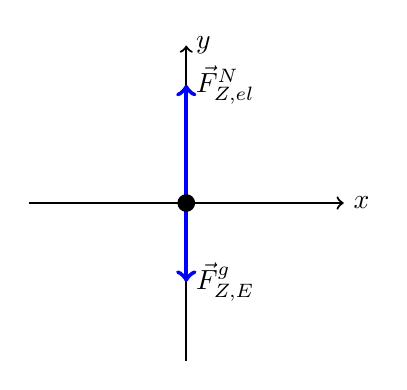
\begin{tikzpicture}
		\FBDaxes{0,0}{0}{axes}
		\FBDvectorXY{axes}{0,1.5}{FN}
		\node[anchor=west] at (FNtip) {$\vec{F}^{N}_{Z,el}$};
		\FBDvectorXY{axes}{0,-1}{FG}
		\node[anchor=west] at (FGtip) {$\vec{F}^{g}_{Z,E}$};
		\FBDdot{axes}
	\end{tikzpicture}
\end{figure}

The floor of the elevator pushes up on Zach with the normal force $\vec{F}^{N}_{Z,el}$. In turn, he pushes back on the floor with an equal and opposite force, $\vec{F}^{N}_{el,Z}$ (this is Newton's 3rd law). If the floor were a scale, this is the force that it would measure---it doesn't magically know the force of gravity on Zach, $\vec{F}^{g}_{Z,E}$ (which some might refer to as Zach's actual weight); it can only go off of what it feels from Zach's feet pushing on it. The normal force is Zach's apparent weight.
}
\ProblemSub{\ApparentWeightB}{
(b) What is Zach's apparent weight before the elevator starts braking?
}
\Solution{\ApparentWeightBSol}{
Before braking, the elevator descends at a constant speed. Therefore
\[
\begin{split}
	F^{net}_{y} & = ma_{y} = 0 \\
	F^{N}_{Z,el} - F^{g}_{Z,E} & = 0 \\
	F^{N}_{Z,el} & = F^{g}_{Z,E} = mg = (80\text{ kg})(9.8\text{ m/s}^{2}) \approx 780\text{ N}.
\end{split}
\]
Zach's apparent weight is 780 N while in an inertial reference frame.
}
\ProblemSub{\ApparentWeightC}{
(c) What is Zach's apparent weight while the elevator is braking?
}
\Solution{\ApparentWeightCSol}{
The elevator must decelerate from 12 m/s to 0 m/s over 3.0 seconds. On average, that means
\[
a_{y} = \frac{\Delta v}{\Delta t} = \frac{12\text{ m/s}}{3.0\text{ s}} = 4.0 \text{ m/s}^{2}.
\]
Now, the net force is nonzero, and we find
\[
\begin{split}
	F^{net}_{y} & = ma_{y} \\
	F^{N}_{Z,el} - F^{g}_{Z,E} & = ma_{y} \\
	F^{N}_{Z,el} & = ma_{y} + F^{g}_{Z,E} = m(a_{y} + g) = (80\text{ kg})(4.0\text{ m/s}^{2} + 9.8\text{ m/s}^{2}) \approx 1100\text{ N}.
\end{split}
\]
Zach's apparent weight is 1100 N while in the braking elevator.
}
\Problem{Steady Block on a Sliding Ramp}{\SteadyBlock}{
A block of mass $m$ sits upon a frictionless ramp (inclined at angle $\theta$) that is being pushed to the right. What must the acceleration of the ramp be to prevent the block from sliding down the surface?
}
\ProblemFig{\SteadyBlockFig}{
\centering
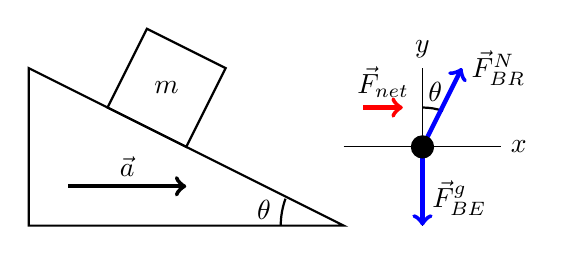
\begin{tikzpicture}
	\draw[thick] (0,0) -- (4,0) -- (0,2) -- cycle;
	\draw[thick] (3.2,0) arc (180:160:1);
	\node[anchor=east] at (3.2,0.2) {$\theta$};
	\draw[thick] (1,1.5) -- (2,1) -- (2.5,2) -- (1.5,2.5) -- cycle;
	\node at (1.75,1.75) {$m$};
	\draw[ultra thick,->] (0.5,0.5) -- (2,0.5);
	\node[anchor=south] at (1.25,0.5) {$\vec{a}$};
	\if\GrayProb1
	\draw (4,1) -- (6,1);
	\node[anchor=west] at (6,1) {$x$};
	\draw (5,0) -- (5,2);
	\node[anchor=south] at (5,2) {$y$};
	\draw[thick] (5,1.5) arc (90:71:0.8);
	\node[anchor=west] at (4.95,1.7) {$\theta$};
	\draw[ultra thick,blue,->] (5,1) -- (5.5,2);
	\node[anchor=west] at (5.5,2) {$\vec{F}^{N}_{BR}$};
	\draw[ultra thick,blue,->] (5,1) -- (5,0);
	\node[anchor=south west] at (5,0) {$\vec{F}^{g}_{BE}$};
	\filldraw[black] (5,1) circle (4pt);
	\draw[ultra thick,red,->] (4.25,1.5) -- (4.75,1.5);
	\node[anchor=south] at (4.5,1.5) {$\vec{F}_{net}$};
	\fi
\end{tikzpicture}
}
\Solution{\SteadyBlockSol}{

If the block is not sliding down the surface of the ramp, then it is moving with it, so the acceleration of the block must be the same as that of the ramp, which points directly to the right. Since we know the direction of acceleration, it will be advantageous to set up our coordinate system with one of the axes along that direction. This differs from several other ramp problems, where a tilted coordinate system is advantageous due to there being fewer vectors to break into components.

If acceleration is along the $x$-axis, as depicted above, we need the two forces (the force on the block normal to the surface of the ramp and the force of gravity on the block) to cancel in the $y$-direction. As such,
\[
0=F^{N}_{BR,y}+F^{g}_{BE,y}=F^{N}_{BR}\cos\theta-mg \implies F^{N}_{BR}\cos\theta=mg \implies F^{N}_{BR}=\frac{mg}{\cos\theta}.
\]
Meanwhile, in the $x$-direction, we only have the $x$-component of the normal force, so
\[
F_{net,x} = F^{N}_{BR,x} = F^{N}_{BR}\sin\theta = mg\frac{\sin\theta}{\cos\theta} = mg\tan\theta.
\]
Since $F_{net,x}=ma_{x}=ma$, we can cancel out the mass to obtain
\[
a = g\tan\theta.
\]
In the special case of a flat ramp, which we expect does not need to move to keep the box from sliding, we have $\theta=0$, and thus $\tan\theta=0$, so our equation indeed gives us $a=0$. Alternatively, if the ramp is vertical, then we cannot keep the block from sliding, as there is nothing beneath it to hold it up. This is the $\theta\to90^{\circ}$ case, and that gives us $a=g\tan\theta\to\infty$, since there is not a finite acceleration sufficient to hold up the block.
}
\Problem[1]{Maximum Tilt}{\MaximumTilt}{
A block is placed on an inclined plane and the angle of the plane is adjusted until the block just begins to slide. The coefficient of static friction is 0.35 and the coefficient of kinetic friction is 0.25.
}
\ProblemSub{\MaximumTiltA}{
(a) Draw a sketch illustrating the problem.
}
\Solution{\MaximumTiltASol}{
\begin{figure}[h]
	\centering
	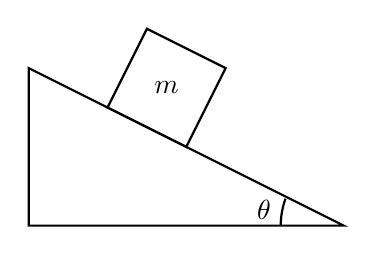
\begin{tikzpicture}
		\draw[thick] (0,0) -- (4,0) -- (0,2) -- cycle;
		\draw[thick] (3.2,0) arc (180:160:1);
		\node[anchor=east] at (3.2,0.2) {$\theta$};
		\draw[thick] (1,1.5) -- (2,1) -- (2.5,2) -- (1.5,2.5) -- cycle;
		\node at (1.75,1.75) {$m$};
	\end{tikzpicture}
\end{figure}
}
\ProblemSub{\MaximumTiltB}{
(b) Draw a free-body diagram for the block. Use the particle model with tilted axes.
}
\Solution{\MaximumTiltBSol}{
\begin{figure}[h]
	\centering
	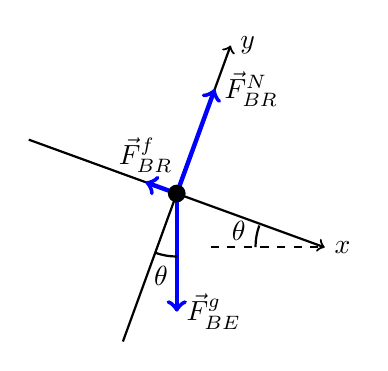
\begin{tikzpicture}
		\FBDaxes{0,0}{-20}{axes}
		\draw[thick,dashed] (1.8,-0.68) -- (0.4,-0.68);
		\draw[thick] (1,-0.68) arc (180:160:0.8);
		\node[anchor=east] at (1,-0.48) {$\theta$};
		\FBDvectorMA{axes}{1.41}{70}{FN}
		\node[anchor=west] at (FNtip) {$\vec{F}^{N}_{BR}$};
		\FBDvectorMA{axes}{0.42}{160}{FF}% 0.49 for static, 0.35 for kinetic
		\node[anchor=south] at (FFtip) {$\vec{F}^{f}_{BR}$};
		\FBDvectorXY{axes}{0,-1.5}{FG}
		\draw[thick] (0,-0.8) arc (270:250:0.8);
		\node[anchor=north] at (-0.2,-0.8) {$\theta$};
		\node[anchor=west] at (FGtip) {$\vec{F}^{g}_{BE}$};
		\FBDdot{axes}
	\end{tikzpicture}
\end{figure}

The diagram is qualitatively accurate for both the static and kinetic friction cases, though the friction vector may vary in size depending on which case we are looking at. Since there are no forces of the same type, I will drop the subscripts for the remainder of the problem (i.e. $F^{g}_{BE}$ will just be $F^{g}$, and so on).
}
\ProblemSub{\MaximumTiltC}{
(c) Find the angle at which the block just begins to slide.
}
\Solution{\MaximumTiltCSol}{
At the maximum angle for which the block doesn't slide, the force of static friction attains its maximum value. Tilting the surface even infinitesimally further, or giving the block the lightest push, will cause it to begin sliding. For now, both the $ x $ and $ y $ components of acceleration are zero. From the $ y $-components, we recover the normal force:
\[
\begin{split}
	F^{net}_{y} & = ma_{y} \\
	F^{N} + F^{g}_{y} & = 0 \\
	(F^{g}_{y} & = -mg\cos\theta) \\
	F^{N} & = -F^{g}_{y} = mg\cos\theta.
\end{split}
\]
This tells us that $ F^{sf}_{max} = \mu_{s}F^{N} = \mu_{s}mg\cos\theta $. We use this in the $ x $-component calculations:
\[
\begin{split}
	F^{net}_{x} & = ma_{x} \\
	F^{g}_{x} - F^{sf}_{max} & = 0 \\
	F^{sf}_{max} & = F^{g}_{x} = mg\sin\theta \\
	\mu_{s}\cancel{mg}\cos\theta & = \cancel{mg}\sin\theta \\
	\mu_{s} & = \frac{\sin\theta}{\cos\theta} = \tan\theta
\end{split}
\]
Now we can solve for the maximum angle:
\[
\theta = \arctan(\mu_{s}) = \arctan(0.35) \approx 19^{\circ} \text{ (2 sig figs)}.
\]
The maximum angle (accounting for significant figures) is 19$ ^{\circ} $, though we should carry the less approximate angle 19.3$ ^{\circ} $ through any further calculations.
}
\ProblemSub{\MaximumTiltD}{
(d) Keeping the angle the same, find the acceleration of the block after it starts to slide.
}
\Solution{\MaximumTiltDSol}{
Now, the friction is kinetic, and therefore it is smaller than the maximum static friction. This results in a net force and acceleration down the plane. The $ y $-component of acceleration is still zero, so we still have $ F^{N} = mg\cos\theta $. In the $ x $ direction, we have
\[
\begin{split}
	a_{x} & = \frac{1}{m} F^{net}_{x} \\
	& = \frac{1}{m} \left(F^{g}_{x} - F^{kf}\right) \\
	& = \frac{1}{m} \left(mg\sin\theta - \mu_{k} F^{N}\right) \\
	& = \frac{1}{m} \left(mg\sin\theta - \mu_{k} mg\cos\theta\right) \\
	& = g \left(\sin\theta - \mu_{k}\cos\theta\right) \\
	& = (9.8\text{ m/s}^{2})(\sin(19.3^{\circ}) - 0.25\cos(19.3^{\circ})) \\
	& \approx 0.93\text{ m/s}^{2}.
\end{split}
\]
}
%\Problem{Suspended Loudspeaker}{\LoudHang}{
A 25 kg loudspeaker is suspended 2.0 m below the ceiling by two cables that are each 30$ ^{\circ} $ from vertical.
}
\ProblemSub{\LoudHangA}{
(a) Draw a sketch illustrating the problem.
}
\Solution{\LoudHangASol}{
\begin{figure}[h]
	\centering
	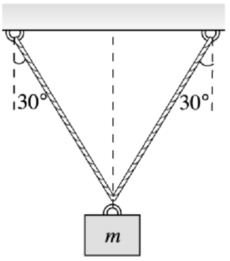
\includegraphics{\FileDepth/Activities/Suspended_Loudspeaker/Two_Cable_Speaker.pdf}
\end{figure}
}
\ProblemSub{\LoudHangB}{
(b) Draw a free-body diagram for the loudspeaker.
}
\Solution{\LoudHangBSol}{
\begin{figure}[h]
	\centering
	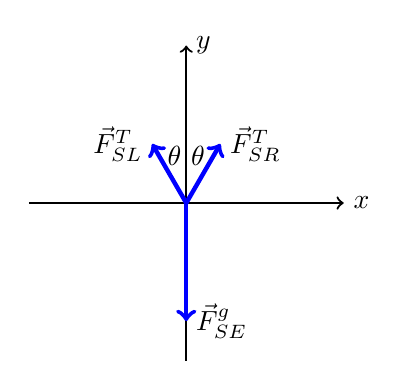
\begin{tikzpicture}
		\FBDaxes{0,0}{0}{axes}
		\FBDvectorMA{axes}{0.866}{60}{RT}
		\node[anchor=west] at (RTtip) {$\vec{F}^{T}_{SR}$};
		\node at (0.15,0.6) {$\theta$};
		\FBDvectorMA{axes}{0.866}{120}{LT}
		\node[anchor=east] at (LTtip) {$\vec{F}^{T}_{SL}$};
		\node at (-0.15,0.6) {$\theta$};
		\FBDvectorXY{axes}{0,-1.5}{FG}
		\node[anchor=west] at (FGtip) {$\vec{F}^{g}_{SE}$};
	\end{tikzpicture}
\end{figure}

Here, $\vec{F}^{T}_{SR}$ is the tension acting on the speaker from the cable on the right, and $\vec{F}^{T}_{SL}$ is the tension acting on the speaker from the cable on the left. Since there is only one object, I will drop the $S$ subscript in further calculations, and since there is only one force of gravity, I will drop both subscripts from it.
}
\ProblemSub{\LoudHangC}{
(c) Find the tension in each cable.
}
\Solution{\LoudHangCSol}{
First, we consider the $ x $-components. The loudspeaker is not accelerating, so
\[
F^{net}_{x} = ma_{x} = 0.
\]
The sum of the forces in this direction is
\[
F^{net}_{x} = F^{T}_{R}\sin\theta - F^{T}_{L}\sin\theta,
\]
therefore
\[
\begin{split}
	F^{T}_{L}\cancel{\sin\theta} & = F^{T}_{R}\cancel{\sin\theta} \\
	F^{T}_{L} & = F^{T}_{R}.
\end{split}
\]
This can be seen in the symmetry of the problem. Now, in the vertical direction, we have
\[
\begin{split}
	F^{net}_{y} & = ma_{y} = 0 \\
	F^{T}_{R}\cos\theta + F^{T}_{L}\cos\theta - F^{g} & = 0 \\
	2F^{T}_{R}\cos\theta - mg & = 0 \\
	F^{T}_{R} & = \frac{mg}{2\cos\theta} \\
	& = \frac{(25\text{ kg})(9.8\text{ m/s}^{2})}{2\cos(30^{\circ})} \\
	& \approx 140\text{ N}.
\end{split}
\]
Each cable has 140 N of tension in it.
}
\end{document}